\documentclass[12pt]{report}
\usepackage[spanish]{babel}
\usepackage[utf8]{inputenc}
\usepackage{amsmath}
\usepackage{amssymb}
\usepackage{amsthm}
\usepackage{graphics}
\usepackage{subfigure}
\usepackage{lipsum}
\usepackage{array}
\usepackage{multicol}
\usepackage{enumerate}
\usepackage[framemethod=TikZ]{mdframed}
\usepackage[a4paper, margin = 1.5cm]{geometry}
\usepackage{tikz}
\usepackage{pgffor}
\usepackage{ifthen}
\usepackage{listings}
\usepackage{hyperref}
\usepackage{xcolor}
\usepackage{enumitem}

%Gestión de Hipervínculos

\hypersetup{
    colorlinks=true,
    linkcolor=black,
    filecolor=magenta,      
    urlcolor=cyan
}

%Gestión de Código de Programación

\definecolor{listing-background}{HTML}{F7F7F7}
\definecolor{listing-rule}{HTML}{B3B2B3}
\definecolor{listing-numbers}{HTML}{B3B2B3}
\definecolor{listing-text-color}{HTML}{000000}
\definecolor{listing-keyword}{HTML}{435489}
\definecolor{listing-keyword-2}{HTML}{1284CA} % additional keywords
\definecolor{listing-keyword-3}{HTML}{9137CB} % additional keywords
\definecolor{listing-identifier}{HTML}{435489}
\definecolor{listing-string}{HTML}{00999A}
\definecolor{listing-comment}{HTML}{8E8E8E}

\lstdefinestyle{myStyle}{
    language         = java,
    alsolanguage     = scala,
    numbers          = left,
    xleftmargin      = 2.7em,
    framexleftmargin = 2.5em,
    backgroundcolor  = \color{gray!15},
    basicstyle       = \color{listing-text-color}\linespread{1.0}\ttfamily,
    breaklines       = true,
    frameshape       = {RYR}{Y}{Y}{RYR},
    rulecolor        = \color{black},
    tabsize          = 2,
    numberstyle      = \color{listing-numbers}\linespread{1.0}\small\ttfamily,
    aboveskip        = 1.0em,
    belowskip        = 0.1em,
    abovecaptionskip = 0em,
    belowcaptionskip = 1.0em,
    keywordstyle     = {\color{listing-keyword}\bfseries},
    keywordstyle     = {[2]\color{listing-keyword-2}\bfseries},
    keywordstyle     = {[3]\color{listing-keyword-3}\bfseries\itshape},
    sensitive        = true,
    identifierstyle  = \color{listing-identifier},
    commentstyle     = \color{listing-comment},
    stringstyle      = \color{listing-string},
    showstringspaces = false,
}

\lstset{style = myStyle}

%Gestión de Marca de Agua

\newcounter{it}
\newcommand*\watermarktext[1]{\begin{tabular}{c}
    \setcounter{it}{1}%
    \whiledo{\theit<100}{%
    \foreach \col in {0,...,15}{#1\ \ } \\ \\ \\
    \stepcounter{it}%
    }
    \end{tabular}
    }

\AddToHook{shipout/foreground}{
    \begin{tikzpicture}[remember picture,overlay, every text node part/.style={align=center}]
        \node[rectangle,black,rotate=30,scale=2,opacity=0.04] at (current page.center) {\watermarktext{Cristo Daniel Alvarado ESFM\quad}};
  \end{tikzpicture}
}

%Redefinición de comandos

\def\proof{\paragraph{Demostración:\\}}
\def\endproof{\hfill$\blacksquare$}

\def\sol{\paragraph{Solución:\\}}
\def\endsol{\hfill$\square$}

%Definición de ambientes

\newtheoremstyle{largebreak}
  {}% use the default space above
  {}% use the default space below
  {\normalfont}% body font
  {}% indent (0pt)
  {\bfseries}% header font
  {}% punctuation
  {\newline}% break after header
  {}% header spec

\theoremstyle{largebreak}

\newmdtheoremenv[
    leftmargin=0em,
    rightmargin=0em,
    innertopmargin=0pt,
    innerbottommargin=5pt,
    hidealllines = true,
    roundcorner = 5pt,
    backgroundcolor = gray!60!red!30
]{exa}{Ejemplo}[section]

\newmdtheoremenv[
    leftmargin=0em,
    rightmargin=0em,
    innertopmargin=0pt,
    innerbottommargin=5pt,
    hidealllines = true,
    roundcorner = 5pt,
    backgroundcolor = gray!50!blue!30
]{obs}{Observación}[section]

\newmdtheoremenv[
    leftmargin=0em,
    rightmargin=0em,
    innertopmargin=0pt,
    innerbottommargin=5pt,
    rightline = false,
    leftline = false
]{theor}{Teorema}[section]

\newmdtheoremenv[
    leftmargin=0em,
    rightmargin=0em,
    innertopmargin=0pt,
    innerbottommargin=5pt,
    rightline = false,
    leftline = false
]{propo}{Proposición}[section]

\newmdtheoremenv[
    leftmargin=0em,
    rightmargin=0em,
    innertopmargin=0pt,
    innerbottommargin=5pt,
    rightline = false,
    leftline = false
]{cor}{Corolario}[section]

\newmdtheoremenv[
    leftmargin=0em,
    rightmargin=0em,
    innertopmargin=0pt,
    innerbottommargin=5pt,
    rightline = false,
    leftline = false
]{lema}{Lema}[section]

\newmdtheoremenv[
    leftmargin=0em,
    rightmargin=0em,
    innertopmargin=0pt,
    innerbottommargin=5pt,
    roundcorner=5pt,
    backgroundcolor = gray!30,
    hidealllines = true
]{mydef}{Definición}[section]

\newmdtheoremenv[
    leftmargin=0em,
    rightmargin=0em,
    innertopmargin=0pt,
    innerbottommargin=5pt,
    roundcorner=5pt
]{excer}{Ejercicio}[section]

%Definición de nuevas funciones

\newcommand\abs[1]{\ensuremath{\left|#1\right|}}
\newcommand\divides{\ensuremath{\bigm|}}
\newcommand\cf[3]{\ensuremath{#1:#2\rightarrow#3}}
\newcommand\contradiction{\ensuremath{\#_c}}
\newcommand\natint[1]{\ensuremath{\left[\big|#1\big|\right]}}
\newcommand{\dom}[1]{\textup{dom}\left(#1 \right)}

\begin{document}
    \setlength{\parskip}{5pt} % Añade 5 puntos de espacio entre párrafos
    \setlength{\parindent}{12pt} % Pone la sangría como me gusta
    \title{Curso de Lógica Matemática
    
    Teoría de la Computabilidad}
    \author{Cristo Daniel Alvarado}
    \maketitle

    \tableofcontents %Con este comando se genera el índice general del libro

    \newpage

    \setcounter{chapter}{2}

    \chapter{Conjuntos y Funciones computables}

    Todo de lo que se va a tratar esta parte es de: ¿Cómo formalizar la noción de \textit{procedimiento mecánico, efectivo} o \textit{sistemático}? Con esto nos referimos a:
    \begin{itemize}
        \item Tener un número finito de instrucciones.
        \item Terminar el procedimiento en un número finito de pasos.
        \item Usar únicamente \textit{papel y lápiz}.
        \item No requiere razonamiento, solo se siguen reglas.
    \end{itemize}

    Básicamente se pretendía que dada una fórmula, encontrar un algoritmo que nos diga si esa fórmula es verdadera o falsa. Básicamente se pretendía formalizar las demostraciones para ver lo que nosotros podemos demostrar únicamente usando los axiomas.

    Turing y Alonzo Church eventualmente se hicieron preguntas en la misma dirección. En la Tesis de Church-Turing se probó que estas tres preguntas en realidad se reducen a un mismo problema.

    \section{Máquinas de Turing}

    \begin{mydef}
        Una \textbf{máquina de Turing} consta de:
        \begin{itemize}
            \item Un \textit{alfabeto}, un conjunto finito $L$.
            \item Un conjunto finito $S$ de \textit{estados}.
            \item Una función parcial $\cf{T}{L^*\times S}{L^*\times S\times\left\{<,-,> \right\}}$ llamada \textit{función de transición}.
        \end{itemize}
        donde $L^*=L\cup\left\{* \right\}$.
    \end{mydef}

    Intuitivamente, uno debe imaginar que esto es una especie de \textit{computadora rudimentaria}. Generalmente esto se conceptualiza como una cinta.

    \begin{center}
        \label{Turing1}
        \begin{figure}
            \begin{center}
                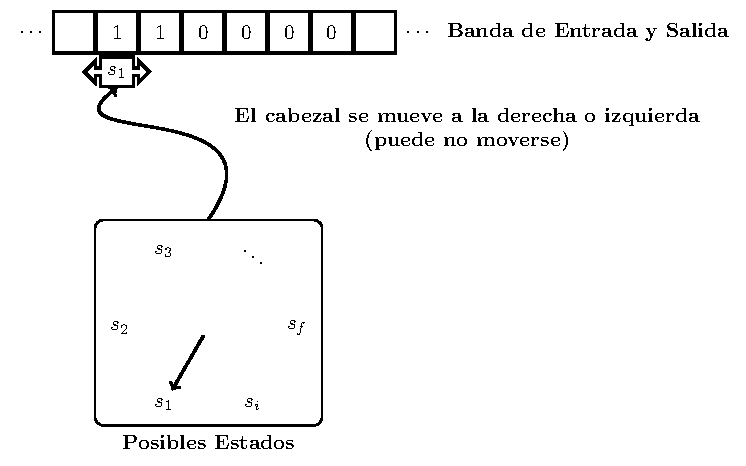
\includegraphics[scale=1]{images/fig_1.pdf}
            \end{center}
            \caption{Ejemplo de Máquina de Turing}
        \end{figure}
    \end{center}

   El cabezal $c$ puede moverse a la derecha, izquierda o no moverse, dependiendo del estado en el que esté. En la Figura \ref{Turing1} se muestra que el hay al menos 5 diferentes estados, desde el estado inicial ($s_i$) hasta el final ($s_f$). Dependiendo de la entrada, la función $T$ nos dirá lo que hará el cabezal, si cambia un elemento de la banda, si se mueve o si cambia de estado (o todas a la vez).

   En este ejemplo, el alfabeto sería $L=\left\{0,1 \right\}$, el conjunto de estados es $S=\left\{s_i,s_1,...,s_f \right\}$ y la función sería representada por lo que sea que haga el cabezal.

    \begin{exa}
        Considere $L=\left\{1 \right\}$, $S=\left\{s_i,s_1,s_2 \right\}$ y,
        \begin{equation*}
            T=\left\{(s_i,*,s_1,*,>),(s_i,1,s_1,1,>),(s_1,1,s_1,1,>),(s_1,1,s_2,1,-) \right\}
        \end{equation*}
        La cinta se ve más o menos así:

    \end{exa}

    Para los siguientes ejercicios, ir a la página: \href{https://turingmachinesimulator.com/}{Simulador Máquina de Turing}.

    \begin{excer}
        Codifique una máquina de Turing que sume 1 a un número dado en binario.
    \end{excer}

    \begin{lstlisting}
        name: Sumar uno en unario
        init: s0
        accept: sf

        
        // Funciones de Transicion

        s0,_
        s0,_,>

        s0,1
        s1,1,-

        s0,0
        s1,0,-

        s1,1
        s1,0,>

        s1,0
        s1,1,>

        s1,_
        sf,_,-

        // < = left
        // > = right
        // - = hold
        // use _ for blank cells

        // States and symbols are case-sensitive

        // Load your code and click COMPILE.
        //  or load an example (top-right).
    \end{lstlisting}

    \begin{excer}
        Codifique una máquina de Turing que dada un número en binario, invierta su orientación, es decir, si la cadena es $(a_1,...,a_n)$, que la máquina de Turing la convierta en $(a_n,...,a_1)$. 
    \end{excer}

    \begin{lstlisting}
        name: invertirCadena
        init: s0
        accept: s1,sf,l,c,u
        
        //esto para que se empiece a mover
        s0,_
        s0,_,>
        
        s0,0
        x,0,<
        
        s0,1
        x,1,<
        
        x,_
        s1,2,>
        
        s1,0
        s1,0,>
        
        s1,1
        s1,1,>
        
        //logica cuando encuentre cosas
        
        s1,_
        s2,_,<
        
        s2,_
        s2,_,<
        
        s2,0
        c00,_,>
        
        s2,1
        u00,_,>
        
        //mueve cosas al inicio
        
        c00,_
        m,0,<
        
        u00,_
        m,1,<
        
        //ya en ciclo
        
        //mueve derecha
        
        m,_
        l,_,<
        
        l,_
        l,_,<
        
        l,0
        c0,_,>
        
        l,1
        u0,_,>
        
        c0,_
        c0,_,>
        
        //mueve izquierda
        
        u0,_
        u0,_,>
        
        c0,0
        c1,0,>
        
        c0,1
        c1,1,>
        
        u0,0
        u1,0,>
        
        u0,1
        u1,1,>
        
        c1,0
        c1,0,>
        
        c1,1
        c1,1,>
        
        u1,0
        u1,0,>
        
        u1,1
        u1,1,>
        
        c1,_
        m,0,<
        
        u1,_
        m,1,<
        
        m,0
        m,0,<
        
        m,1
        m,1,<
        
        l,2
        sf,_,>
        
        sf,_
        sf,_,>
        
        sf,0
        sff,0,-
        
        sf,1
        sff,1,-        
    \end{lstlisting}

    \begin{mydef}
        Una función $f$ es \textbf{computable} si:
        \begin{enumerate}[label = \textit{(\arabic*)}]
            \item $\dom{f}\subseteq\mathbb{N}$.
            \item Existe un algoritmo tal que para cada $n\in\mathbb{N}$, el algoritmo al correrse con $n$ como argumento, se detiene en tiempo finito si y sólo si $n\in\dom{f}$ y en tal caso arroja $f(n)$ como salida. 
        \end{enumerate}
    \end{mydef}

    ¿Qué es un algoritmo? Resulta que hay muchas formas de definirlo, sin embargo, nosotros adoptaremos la siguiente definición:

    \begin{mydef}
        Un \textbf{algoritmo} lo interpretaremos como una máquina de Turing.
    \end{mydef}

    \begin{obs}
        Un algoritmo también puede verse como un código en C, C++, Python o \LaTeX (usando las librerías adecuadas).
    \end{obs}

    En la Tesis de Church-Turing, cualquier noción es equivalente.

    \begin{obs}
        De ahora en adelante consideraremos a los naturales con el 0.
    \end{obs}

    \begin{exa}
        La función $\cf{f}{\mathbb{N}\setminus\left\{0,1\right\}}{\mathbb{N}}$ tal que $n\mapsto\min\left\{p\in\mathbb{N}\Big|p\textup{ es primo y }p\divides n \right\}$ es computable.
    \end{exa}

    \begin{proof}
        Se tiene el siguiente algoritmo:
        \begin{lstlisting}
int f(int n){
    for(int k = 2;n % k != 0;k++) return k;
}
        \end{lstlisting}
    \end{proof}

    \begin{exa}
        Considere la función $\cf{g}{\left\{n^2\Big|n\in\mathbb{N} \right\}}{\mathbb{N}}$ dada por $n^2\mapsto n$. Esta función es computable.
    \end{exa}

    \begin{proof}
        Se tiene el siguiente algoritmo:
        \begin{lstlisting}
int g(int m){
    for(int k = 0;k*k != m;k++) return k;
}
        \end{lstlisting}
    \end{proof}

    \begin{exa}
        La función $\cf{+}{\mathbb{N}\times\mathbb{N}}{\mathbb{N}}$ es computable.
    \end{exa}

    \begin{proof}
        Recordemos que existe una biyección entre $\mathbb{N}\times\mathbb{N}$ y $\mathbb{N}$ dada por:
        \begin{equation*}
            (k,l)\mapsto 2^k(2l+1)
        \end{equation*}
        por lo cual, podemos ver a la función suma como una función de $\mathbb{N}$ en $\mathbb{N}$.
    \end{proof}

    \begin{obs}
        Podemos ir más allá en el ejemplo anterior, podemos generalizar la idea anterior usando conjuntos que puedan ser representados mediante números naturales (recuerde la enumeración de Gödel).
    \end{obs}

    Veremos más ejemplos que nos ayudarán más adelante a hacer cosas más complejas:

    \begin{itemize}
        \item La función sucesor (se vió en un ejercicio anterior).
        \item Cualquier función constante.
        \item La $i$-ésima proyección de una $k$-tupla.
    \end{itemize}
    \begin{lstlisting}
int p_2(int a, int b, int c){
    return b;
}
    \end{lstlisting}
    este ejemplo anterior es la 2-ésima proyección de una 3-tupla.

    \begin{exa}
        La función exponencial: $(a,b)\mapsto a^{b}$ es computable.
    \end{exa}

    \begin{proof}
        En efecto, se tiene el siguiente algoritmo:
        \begin{lstlisting}
int exp(int a, int b){
    if(b==0){
        return 1;
    }
    else return a*exp(a,b-1);
}
        \end{lstlisting}
    \end{proof}

    \begin{exa}
        La función factorial $n\mapsto n!$ es computable.
    \end{exa}

    \begin{proof}
        En efecto, se tiene el siguiente algoritmo:
        \begin{lstlisting}
int fact(int n){
    if(n==0) return 1;
    else return n*fact(n-1);
}
        \end{lstlisting}
    \end{proof}

    \begin{exa}
        Las funciones máximo y mínimo son computables.
    \end{exa}

    \begin{exa}
        El algoritmo de la división es computable.
    \end{exa}

    \begin{proof}
        En efecto, se tiene el siguiente algoritmo:
        \begin{lstlisting}
int div(int a, int b){
    for(int i=1; i*b<=a;i++){} //se queda y acaba si es que se puede dividir
    q = i-1;
    r = a-b*q;
    return exp(2,q)*(2*r-1); //codificamos de esta manera la salida del programa
}
        \end{lstlisting}
    \end{proof}

    \begin{obs}
        Cuando coloquemos $\cf{f}{;A}{B}$, entenderemos que $\dom{f}\subseteq A$, es decir que $f$ es una función parcial.
    \end{obs}

    \begin{theor}
        Sea $\cf{f}{;\mathbb{N}^k}{\mathbb{N}}$ una función computable, y sean $\cf{g_1,...,g_k}{;\mathbb{N}}{\mathbb{N}}$ funciones computables. Entonces:
        \begin{enumerate}[label = \textit{(\arabic*)}]
            \item La función $\cf{h_1}{;\mathbb{N}}{\mathbb{N}}$ dada por: $h_1(x)=f(g_1(x),\cdots,g_k(x))$ es computable.
            \item La función $\cf{h_2}{;\mathbb{N}^{ k-1}}{\mathbb{N}}$ dada por:
            \begin{equation*}
                h_2(x_2,\cdots,x_k)=(\mu x)(f(x,x_2,\cdots,x_k)=0)
            \end{equation*}
            donde la función $\mu x$ es el mínimo de $x$ tal que lo de adentro se hace 0, siendo $f$ tal que para todo $i\leq x$, $f(i,x_2,...,x_k)$ está bien definido, también es computable.
        \end{enumerate}
    \end{theor}

    \begin{proof}
        De \textit{(1)}: Considere el algoritmo:
        \begin{lstlisting}
int h_1(int x){
    int y_1 = g_1(x);
    int y_2 = g_2(x);
    ...
    int y_k = g_k(x);
    return f(y_1,...,y_k);
}
        \end{lstlisting}
    \end{proof}
    es una función computable, ya que si no puede calcular algún valor, se queda atorado.

    De \textit{(2)}: Considere el algoritmo:
    \begin{lstlisting}
        int h_2(int x_2,...,int x_k){
            for(int x=0; f(x,x_2,...,x_k)!=0;x++) return x;
        }
    \end{lstlisting}
    es de una función computable.

    \begin{mydef}
        Una función computable $\cf{f}{;\mathbb{N}^k}{\mathbb{N}}$ es \textbf{total}, si $\dom{f}=\mathbb{N}^k$. En computabilidad esto se denota por:
        \begin{equation*}
            (\forall x_1,...,x_k)(f(x_1,...,x_k)\downarrow)
        \end{equation*}
        esto es, que para cualquier entrada $f$ está bien definida.
    \end{mydef}

    \begin{obs}
        En el teorema anterior, siempre se puede hacer (2) si la función $f$ es total.
    \end{obs}

    \begin{excer}
        Codifique una máquina de Turing que sume dos números en binario.
    \end{excer}

    \begin{lstlisting}
name: suma_numeros_binario
init: s0
accept: sf

s0,_
s0,_,>

s0,0
s1,0,>

s1,0
s1,0,>

s0,1
s1,1,>

s1,1
s1,1,>

//operaciones de suma

//el estado s_s0 nos dice que va a empezar a contar el otro numero
//el estado s_s1 nos dice que encontro un numero positivo para sumar

s1,+
s_s0,+,>

s_s0,0
s_s0,0,>

s_s0,1
s_s1,1,>

s_s1,1
s_s1,1,>

s_s1,0
s_s1,0,>

//llego al final de la cadena

s_s1,_
sr0,_,<

sr0,1
srf,0,>

sr0,0
sr0,0,<

srf,0
srf,1,>

srf,_
ss0,_,<

//ss es que ahora le va sumar uno a la cadena de la izquierda

ss0,0
ss0,0,<

ss0,1
ss0,1,<

ss0,+
ss1,+,<

ss1,0
s1,1,>

ss1,1
ss1,0,<

ss1,_
s1,1,>

//cuando no haya nada por sumar, simplemente se detiene

s_s0,_
sf0,_,<

sf0,0
sf0,_,<

sf0,+
sf,_,-

// < = left
// > = right
// - = hold
// use underscore for blank cells

//States and symbols are case-sensitive

//Load your code and click COMPILE.
//or load an example (top-right).
    \end{lstlisting}

    \begin{excer}
        Codifique una máquina de Turing que sume dos números en binario.
    \end{excer}

\begin{lstlisting}
name: resta_numeros_1
init: s0
accept: sf

s0,_
s0,_,>

s0,0
s1,0,>

s1,0
s1,0,>

s0,1
s1,1,>

s1,1
s1,1,>

//operaciones de resta

//sr0 es estado resta inicial

//srf es estado resta final

s1,_
sr0,_,<

sr0,1
srf,0,>

sr0,0
sr0,0,<

srf,0
srf,1,>

srf,_
sf,_,-

// < = left
// > = right
// - = hold
// use underscore for blank cells

//States and symbols are case-sensitive

//Load your code and click COMPILE.
//or load an example (top-right).
\end{lstlisting}

\begin{excer}
    Dada una cadena en binario, escribir un programa que haga una copia de la misma.
\end{excer}

\begin{lstlisting}
name: copiar_cadena
init: s0
accept: sf

//se empieza a mover y marca el inicio de la cadena

s0,_
s0,_,>

s0,0
s1,0,<

s2,0
s2,0,>

s0,1
s1,1,<

s2,1
s2,1,>

s1,_
s2,|,>

s2,0
s2,0,>

s2,1
s2,1,>

//coloca el inicio de la copia de la cadena

s2,_
sd,c,<

sd,0
sd,0,<

sd,1
sd,1,<

sd,2
sd,2,<

sd,3
sd,3,<

sd,c
sd,c,<

sd,|
sdp,|,>

//deteccion de si es 0 o 1

sdp,0
sdp0,2,>

sdp,1
sdp1,3,>

sdp,2
sdp,2,>

sdp,3
sdp,3,>

//movimiento a la derecha para colocar 0 o 1

sdp0,0
sdp0,0,>

sdp0,1
sdp0,1,>

sdp1,0
sdp1,0,>

sdp1,1
sdp1,1,>

//detecta la copia

sdp0,c
sdp0,c,>

sdp1,c
sdp1,c,>

sdp0,_
sd,0,<

sdp1,_
sd,1,<

//detecta que ya debe terminar

sdp,c
scam,c,<

scam,2
scam,0,<

scam,3
scam,1,<

scam,|
sf,_,-
\end{lstlisting}

\begin{excer}
    Programar una máquina de Turing que haga el producto de dos números. 
\end{excer}

\begin{lstlisting}
name: producto_numeros
init: p0
accept: pf

//input: [n]_2*[m]_2

//empieza el movimiento

p0,_
p0,_,>

p0,0
p1,0,<

p0,1
p1,1,<

p1,_
p2,|,>

p2,0
p2,0,>

p2,1
p2,1,>

p2,*
p2,*,>

//llego al final de la cadena

p2,_
sd,c,<

//PARTE PRIMERA COPIA

sd,0
sd,0,<

sd,1
sd,1,<

sd,2
sd,2,<

sd,3
sd,3,<

sd,*
sd,*,<

sd,c
sd,c,<

sd,|
sdp,|,>

//deteccion de si es 0 o 1

sdp,0
sdp0,2,>

sdp,1
sdp1,3,>

sdp,2
sdp,2,>

sdp,3
sdp,3,>

sdp,c
sdp,c,>

//movimiento a la derecha para colocar 0 o 1

sdp0,0
sdp0,0,>

sdp0,1
sdp0,1,>

sdp1,0
sdp1,0,>

sdp1,1
sdp1,1,>

//detecta la copia

sdp0,*
sdp0,*,>

sdp1,*
sdp1,*,>

sdp0,c
sdp0,c,>

sdp1,c
sdp1,c,>

sdp0,_
sd,0,<

sdp1,_
sd,1,<

//detecta que ya debe terminar y elimina los cambios que hizo

sdp,*
scam,*,<

scam,2
scam,0,<

scam,3
scam,1,<

scam,|
sf,_,>

//segunda copia

sf,0
sf,0,>

sf,1
sf,1,>

sf,*
sf,*,>

sf,c
sf,c,>

//ahora, hace la segunda copia

//coloca el inicio de la copia de la cadena

sf,_
rd,d,<

rd,0
rd,0,<

rd,1
rd,1,<

rd,2
rd,2,<

rd,3
rd,3,<

rd,d
rd,d,<

rd,c
rdp,c,>

//deteccion de si es 0 o 1

rdp,0
rdp0,2,>

rdp,1
rdp1,3,>

rdp,2
rdp,2,>

rdp,3
rdp,3,>

//movimiento a la derecha para colocar 0 o 1

rdp0,0
rdp0,0,>

rdp0,1
rdp0,1,>

rdp1,0
rdp1,0,>

rdp1,1
rdp1,1,>

//detecta la copia

rdp0,d
rdp0,d,>

rdp1,d
rdp1,d,>

rdp0,_
rd,0,<

rdp1,_
rd,1,<

//detecta que ya debe terminar

rdp,d
rcam,d,<

rcam,2
rcam,0,<

rcam,3
rcam,1,<

rcam,c
rf,c,<

rf,0
rf,0,<

rf,1
rf,1,<

rf,*
rf,*,<

//ahora ya puede empezar a sumar uno por uno

rf,_
rs,_,>

rs,0
rs,0,>

rs,1
rs,1,>

rs,*
rs,*,>

rs,c
rs,c,>

rs,d
rs,d,>

//hace la primera suma

rs,_
rsr,_,<

rsr,1
rss,0,>

rss,0
rss,1,>

rss,_
Rf,_,<

//en Rf

Rf,0
Rf,0,<

Rf,1
Rf,1,<

Rf,c
Rf,c,<

Rf,d
Rf,d,<

//ahora, si detecta el * es pq ahora tiene que sumar

Rf,*
estSum,*,<

estSum,0
estSumAcaba,1,>

estSum,_
estSumAcaba,1,>

estSum,1
estSum,0,<

//aqui acabo de sumar

rsr,0
RF,0,-

//se mueve para ahora sumar a la otra cadena    
    \end{lstlisting}

    \begin{mydef}
        Un conjunto $X$ es \textbf{computable}, si puede ser visto como input de elementos de $\mathbb{N}$, y su función característica es computable.
    \end{mydef}
    
    \begin{exa}
        Sea $\cf{F}{\mathbb{N}}{\mathbb{N}}$ la función:
        \begin{equation*}
            F(n)=\left\{
                \begin{array}{lcr}
                    1 & \textup{si} & \textup{conjetura Gölbach es verdadera.}\\
                    0 & \textup{ en } & \textup{caso contrario.}\\
                \end{array}
            \right.
        \end{equation*}
        esta función es computable.
    \end{exa}

    \begin{exa}
        La funcion $\cf{f}{\mathbb{N}}{\mathbb{N}}$ tal que:
        \begin{equation*}
            f(n)=\min\left\{p\Big|p>n\textup{ y tanto }p\textup{ como }p+2\textup{ son primos}\right\}
        \end{equation*}
        en efecto, se tiene el siguiente algoritmo de $f$:
    \end{exa}

    \begin{lstlisting}
int f(int n){
    for(int i=n+1; i no es primo || i+2 tampoco lo es; i++){
        return i;
    }
}
    \end{lstlisting}

    \section{Máquina Universal de Turing}

    En general, los input de mis algoritmos son $\mathbb{N}$, pero podemso también codificar parejas por medio de números naturales, por lo que realmente también podemos introducir tuplas de $\mathbb{N}^k$.

    \begin{obs}
        Una máquina de Turing es un conjunto finito $\left\{a_1,...,a_n \right\}$, donde $a_i=(s_{i_1},t_{i_2},s_{i_3},t_{i_4},l)$ con $l\in\left\{<,-,> \right\}$. Podemos hacer una codificación estas 6-tuplas:
        \begin{center}
            \begin{tabular}{l | c | r}
                0 & - & 0 \\
                1 & - & | \\
                2 & - & * \\
                3 & - & > \\
                \vdots & - & \vdots \\
            \end{tabular}
        \end{center}
        en este caso, codificamos elementos de $\left[\left\{0,1,*,<,>,-,s_1,...,s_n \right\}^k\right]^{<\aleph_0}$ (cadenas finitas de tuplas finitas). Lo que podemos hacer enotnces es codificar máquinas de Turing.
    \end{obs}

    \begin{theor}
        El conjunto
        \begin{equation*}
            \left\{x\in X\Big|x\textup{ es máquina de Turing} \right\}
        \end{equation*}
        y,
        \begin{equation*}
            \left\{n\in\mathbb{N}\Big|n\textup{ codifica una máquina de Turing} \right\}
        \end{equation*}
        son computables.
    \end{theor}

    \begin{proof}
        Ver simulador de máquina de Turing.
    \end{proof}
    
    \begin{mydef}
        Denotaremos la \textbf{máquina universal de Turing} por $\varphi$, donde
        \begin{equation*}
            \cf{\varphi}{;\mathbb{N}^2}{\mathbb{N}}
        \end{equation*}
        dada por $\varphi(e,n)$ es el resultado de correr la $e$-ésima máquina de Turing con input $n$.
    \end{mydef}

    \begin{obs}
        $\varphi$ es una función computable.
    \end{obs}

    Una forma de interpretar a $\varphi$ es el simulador de máquina de Turing, pues en este simulador introducimos una máquina de Turing y un input, así que nuestro código sería $e$ y el input sería $n$.
    
    \begin{mydef}
        La función $\cf{\varphi(e,-)}{\mathbb{N}}{\mathbb{N}}$ tal que $n\mapsto\varphi(e,n)$ es llamada la \textbf{$e$-ésima función computable}.
    \end{mydef}

    \begin{theor}[\textbf{Lema del Relleno}]
        Para cada función computable $f$, existen una infinidad de $e\in\mathbb{N}$ tales que $f=\varphi(e,-)$.
    \end{theor}

    Existen funciones que no son computables.

    \begin{obs}
        Como se pueden enumerar todas las funciones computables, el conjunto:
        \begin{equation*}
            \abs{\left\{\cf{f}{\mathbb{N}}{\mathbb{N}}\Big|\textup{ f es computable}\right\}}=\aleph_0
        \end{equation*}
        pero,
        \begin{equation*}
            \abs{\left\{\cf{f}{\mathbb{N}}{\mathbb{N}}\Big|f\textup{ es función} \right\}}=\aleph_1
        \end{equation*}
    \end{obs}

    \begin{exa}
        Se define la función \textbf{Busy Beaver}, $\cf{\sigma}{\mathbb{N}}{\mathbb{N}}$ dada por:
        \begin{equation*}
            \sigma(n)=\max\left\{\textup{output en unario de una máquina de Turing con }\leq n+1\textup{ estados e input }0 \right\}
        \end{equation*}
        de forma inmediata se tiene que $\sigma(0)=1$, ya que solo hay una máquina de Turing con un estado (el estado final), y el mayor output que puede hacer es 1.
    \end{exa}

    \begin{excer}
        Verifique que $\sigma(2)\geq4$.
    \end{excer}

    \begin{theor}
        Si $\cf{f}{\mathbb{N}}{\mathbb{N}}$ es cualquier función computable, entonces existe $N\in\mathbb{N}$ tal que para todo $n\geq N$ se cumple que $f(n)< \sigma(n)$. En particular, \textbf{$\sigma$ no es computable}.
    \end{theor}

    \begin{proof}
        Sea $f$ computable, entonces la función $\cf{g}{;\mathbb{N}}{\mathbb{N}}$ dada por:
        \begin{equation*}
            g(n)=\min\left\{f(2n),f(2n+1) \right\}+1
        \end{equation*}
        también es computable. Por lo tanto, existe alguna máquina de Turing $T$ que calcula a $g$ en unario. Sea $k$ el número de estados (además del estado inicial) de dicha máquina.

        Consideremos la función 
    \end{proof}

    \section{Conjuntos y Relaciones Computables}

    \begin{mydef}
        Un conjunto $X\subseteq\mathbb{N}$ es \textbf{computable} si su función característica $\chi_X$ es computable.
    \end{mydef}

    \begin{exa}
        Los siguientes son conjuntos computables:
        \begin{enumerate}[label = \textit{(\arabic*)}]
            \item $\mathbb{N}$.
            \item $\emptyset$.
            \item $\left\{n\in\mathbb{N}\Big|n\textup{ es cuadrado perfecto} \right\}$.
            \item $\left\{p\in\mathbb{N}\Big|p\textup{ es primo} \right\}$.
            \item $\left\{(n,m)\in\mathbb{N}^2\Big|n\divides m \right\}$.
        \end{enumerate}
    \end{exa}

    \begin{sol}
        En efecto, se tienen los siguientes algoritmos de cada una de las funciones características de los conjuntos anteriores:
        \begin{lstlisting}
int uno(int n) return 1;

int dos(int n) return 0;

int tres(int n){
    for(int i=0; i*i<n;i++){
        if(i*i=n) return 1;
    }
    return 0;
}
        \end{lstlisting}
    \end{sol}

    \begin{propo}
        Sean $X,Y\subseteq\mathbb{N}$ conjuntos computables, entonces $X\cap Y$, $X\cup Y$ y $X\setminus Y$ son también computables (en otras palabras, el conjunto de conjuntos computables es un álgebra booleana).
    \end{propo}

    \begin{proof}
        Basta con ver que:
        \begin{itemize}
            \item $\chi_X(n)\chi_Y(n)=\chi_{ X\cap Y}(n)$.
            \item $\chi_{ X\cup Y}(n)=\max\left\{\chi_X(n),\chi_Y(n) \right\}$.
            \item $\chi_{ X\setminus Y}(n)=\max\left\{1-\chi_X(n),0 \right\}$.
        \end{itemize}
        para todo $n\in\mathbb{N}$.
    \end{proof}

    \begin{theor}
        El conjunto
        \begin{equation*}
            \left\{e\in\mathbb{N}\Big|\varphi(e,-)\textup{ es una función total} \right\}
        \end{equation*}
        no es computable.
    \end{theor}

    \begin{proof}
        En caso contrario, se tendría que la funcioń $h:n\mapsto n$-ésima máquina de Turing que induce una función total, también sería computable (ya que la característica detecta si una función computable es total o no, luego en particular existe una función que codifica a todas las funciones totales).

        Se sigue así que la función $\cf{u}{;\mathbb{N}^2}{\mathbb{N}}$:
        \begin{equation*}
            (x,y)\mapsto \varphi(h(x),y)
        \end{equation*}
        sería total computable. Así que, la función $g(n)=u(n,n)+1$ también es total computable.

        Por ende, existe $m\in\mathbb{N}$ tal que $g=\varphi(h(m),-)$, entonces:
        \begin{equation*}
            \begin{split}
                u(m,m)&=g(m)\\
                &=u(m,m)+1\\
            \end{split}
        \end{equation*}
        lo cual es una contradicción.
    \end{proof}

    \begin{theor}[\textbf{Halting Problem, Enschleidung problem}]
        El conjunto
        \begin{equation*}
            H=\left\{(e,n)\Big|\varphi(e,n)\textup{ está definido} \right\}
        \end{equation*}
        (esto es que $(e,n)\in\dom g$ también denotado por $(e,n)\downarrow$) no es computable.
    \end{theor}

    \begin{proof}
        Supongamos que sí lo es, entonces el conjunto
        \begin{equation*}
            D=\left\{e\in\mathbb{N}\Big|(e,e)\downarrow \right\}
        \end{equation*}
        es computable. Definimos la siguiente función $\cf{f}{;\mathbb{N}}{\mathbb{N}}$ con algoritmo:
        \begin{lstlisting}
int f(int n){
    int i;
    if(chi_X(n)) while(1) i++;
    return 1;
}
        \end{lstlisting}
        claramente esta función es computable, y está definida si $n\notin D$ (en caso contrario, se sigue y ejecuta el programa infinitamente). Por ser computable, existe $e\in\mathbb{N}$ tal que $f=\varphi(e,-)$. Se tiene:
        \begin{equation*}
            \begin{split}
                f(e) \textup{ está definido}&\textup{ si y sólo si }e\notin D \\
                &\textup{ si y sólo si }\varphi(e,e)\textup{ no está definido} \\
                &\textup{ si y sólo si }f(e)\textup{ no está definido}\\
            \end{split}
        \end{equation*}
        lo cual es una contradicción. Por tanto, el conjunto anterior no puede ser computable.
    \end{proof}

    \begin{obs}
        El teorema anterior se conoce como el \textbf{brinco de Turing} y es llamado \textbf{el problema de la detección}.
    \end{obs}

    \begin{obs}
        Del teorema anterior se deduce de forma inmediata que el conjunto
        \begin{equation*}
            D=\left\{e\in\mathbb{N}\Big|\varphi(e,e)\textup{ está definido} \right\}
        \end{equation*}
        no es computable.
    \end{obs}

    \begin{exa}
        El problema 10 de Hilbert.
    \end{exa}

    \chapter{Teoremas de Completud}


\end{document}